\section{Motivation}

Die Gravitationskonstante $g$ bestimmt ohne Zweifel unser Leben.
Sie bestimmt, wie schnell Objekte nahe der Erdoberfläche richtung Erde beschleunigt werden.
Diese konstante ist ausschlaggebend für viele Esenzielle berechnungen, beispielsweise in der Mechanik.
Es lässt sich unter anderem die Fluchtgeschwindigkeit der Erde berechnen welche den Grundstein für
die Raumfahrt legt. Deshalb ist eine exakte Messung dieser konstante von großer Bedeutung und dieser Versuch
vermittelt, mit welchen Methoden dieser exakt bestimmt werden kann.


\section{Messverfahren}
Es wurde ein Pendel an einer Aufhängung mit einer vertikalen und einer horizontalen Skala befestigt.
Zunächst wird die Länge des Pendels bestimmt und die Periodendauer grob bestimmt.
Dafür wurde das Pendel 5 mal 20 Perioden geschwungen und die Zeit bestimmt.
Daraus lässt sich, jedoch ungenau, $g$ bestimmen.\\
Mithilfe dieser Periodendauer konnte die Anzahl an Schwingungen bestimmt werden,
ab welchen die Reaktionszeit vernachlässigbar wird.
Anschließend wurde dese Anzahl an Schwingungen gemessen und die abnahme der Amplitude abgelesen.
Daraus lassen sich die Dämpfungsfaktoren des Pendels bestimmen und anschließend $g$ mit hoher Genauigkeit berechnen.

\section{Grundlagen aus der Physik}

\subsection{Klassisches Fadenpendel}
In einem klassischen Fadenpendel enspricht die Tangentialbeschleunigung genau dem Tangentialanteil der Gravitationskraft.
Für kleine Auslenkungen gilt hier $\sin(\varphi) \approx \varphi$.
Teilt man die erhaltene Gleichung durch $l$ als Fadenlänge ergibt sich mit $\varphi$ als Winkelauslenkung die Differentialgleichung:
\begin{equation}
    \ddot{\varphi} + \frac{g}{l} \varphi = 0
    \label{eq:ho}
\end{equation}

Für die Lösung dieser gilt eine harmonische Schwingung mit Eigenfrequenz $\omega = \tfrac{g}{l}$.
Damit gilt für die Periodendauer $T_0$:

\begin{equation}
    T_0 = 2\pi \sqrt{\frac{l}{g}}
    \label{eq:Tnorm}
\end{equation}
Damit gilt für $g$:
\begin{equation}
    g = 4\pi^2 \frac{l}{T_0^2}
\end{equation}

\subsection{Physikalisches Pendel}

Im physikalischen Pendel lassen sich die bremsenden Faktoren nicht mehr vernachlässigen.
Ebenfalls gilt $\sin(\varphi) \approx \varphi$ nicht mehr. Die Periodendauer ist nun abhängig von der Amplitude.
Es ensteht eeine Verlängerung der Periodendauer:
\begin{equation}
    T^2= T_0^2(1 + \frac{\varphi_0^2}{8})
\end{equation}
Hierbei ist $\varphi_0$ der Winkel ab dem die lineare Näherung aufgrund von hohen Auslenkungen nicht mehr angenommen werden kann.
Dieser berechnet sich durch:
\begin{equation}
    \varphi_0 = \arctan\left(\frac{2\overline{x}}{l}\right)
    \label{eq:phi}
\end{equation}

Wobei $\overline{x}$ die mittlere Aplitude ist und $l$ die Pendellänge.

\subsection{Dämpfung durch Reibung}
Die Funktion der Ampliduden $x(t)$ mit Ausgangsamplitude $x_0$  enhält den Dämpfungskoeffizienten $\delta$.
Dieser gibt die Dämpfung durch die entstehende Reibung an.
\begin{equation}
    x(t) = x_0 e^{-\delta t}
\end{equation}

Davon lässt sich der Einfluss auf die Periodendauer ermitteln. Dabei ist $\omega_0$ die Frequenz des Pendels ohne Reibung.

\begin{equation}
    T_2 = T_1(1+ \frac{\delta ^2}{\omega_0 ^2})
\end{equation}

\subsection{Trägheitsmoment}

In einem physikalischen Pendel spielt das Drehmoment der Kugel und das des Fadens eine entscheidende Rolle.
Dafür wird der Faden als Zylinder mit Höhe $l'$ betrachtet. Damit ergibt sich unter zuhilfenahme des Steinerschen Satzes das Gesamtdrehmoment:
\begin{equation}
    J = J_{Kugel} + J_ {Faden} + m_K l^2
\end{equation}

Mithilfe des Trägheitsmoments kann die Periodendauer des realen Pendels bestimmt werden.

\begin{equation}
    T = 2 \pi \sqrt{\frac{J}{D}}
\end{equation}

Dafür benötigt man allerdings die Winkelrichtgröße $D$ für diese gilt:

$M = -D \varphi$
mit $M$ als Drehmoment.
Dafür wird zuerst wieder $\sin(\varphi) \approx \varphi$ genähert, welches nach obiger Gelichung zum Schluss korigiert wird.
DAnn lässt sich $D$ berechnen.
\begin{equation}
    D = m_K g l \left( 1 - \left(\frac{\rho_L}{\rho_K}- \frac{m_F}{2 m_K}\right)\right)
\end{equation}

Setzt man diese ganzen Korrekturen zusammen ergibt sich mit dem einsetzen der Trägheitsmomente eine abschließende Gleichung für $g$:

\begin{equation}
    g = 4 \pi^2 \frac{l}{T_0^2}\left(1 + \frac{2 r^2}{5l^2}+  \frac{\rho_L}{\rho_K}- \frac{m_F}{2 m_K} + \frac{\delta^2}{\omega_0 ^2} +\frac{\varphi_0^2}{8}\right)
    \label{eq:leckmich}
\end{equation}
\newpage
\section{Aufbau}

\begin{figure}[h!]
    \centering
    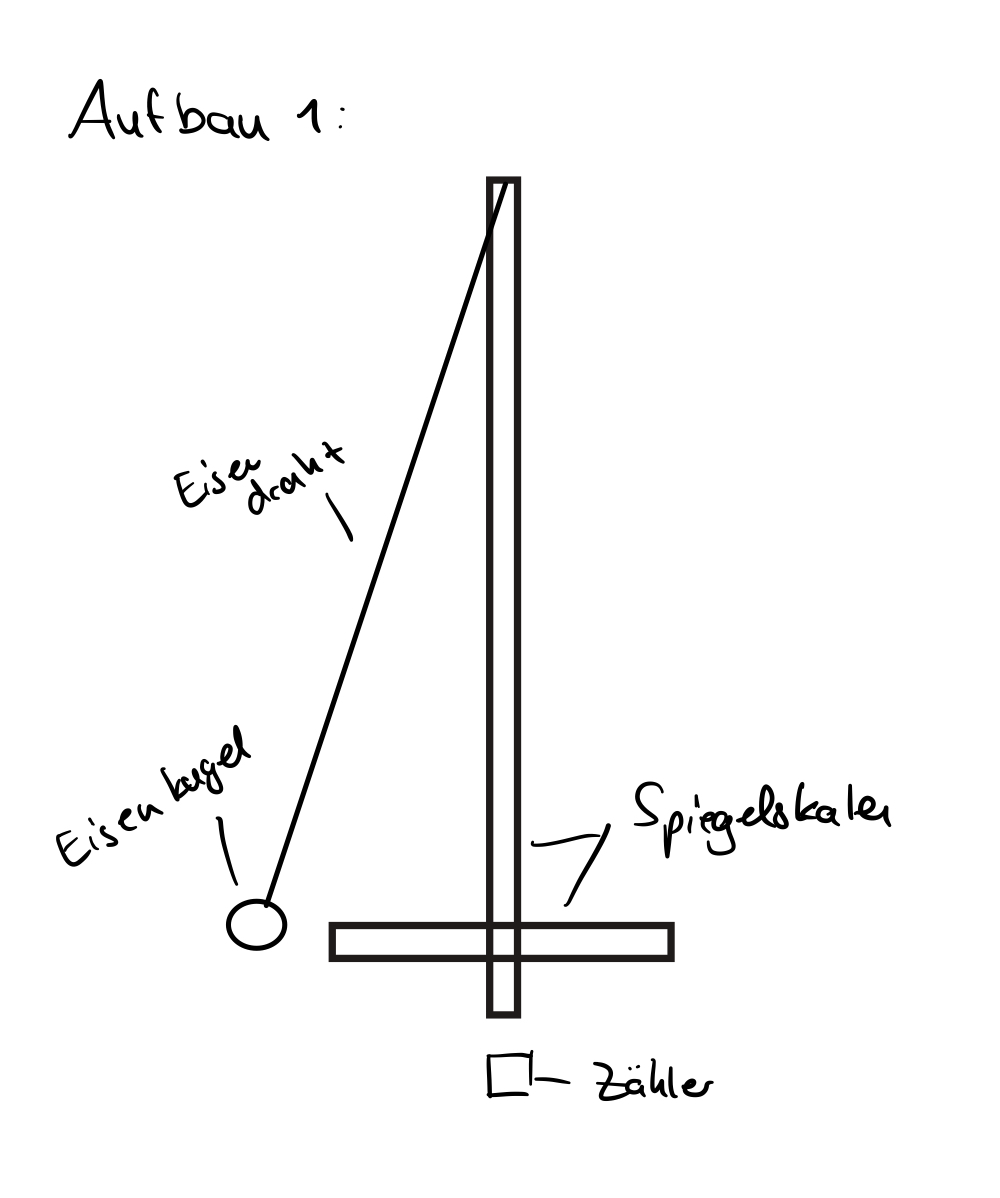
\includegraphics[width = .5\textwidth]{JPEG image-433E-B9B9-77-0.jpeg}
    \caption{Aufbau}
\end{figure}
\clearpage